\lab{Algorithms}{Krylov Subspaces}{Finding Eigenvalues Using Iterative Methods}
\label{lab:kry_arnoldi}

\objective{Discuss simple Krylov Subspace Methods for finding eigenvalues and show some interesting applications.}

Krylov Subspace Methods are widely considered some of the most succesful numerical methods ever invented.
They are simple and robust iterative methods that can be used to find approximate solutions to linear systems and eigenvalue problems involving extremely large matrices.
One of the things that makes these numerical methods so succesful is that they do not require copies or modifications of the original matrix.
Krylov subspace methods are used to estimate some properties of a matrix based on how it acts on vectors through matrix multiplication.
This is especially useful for matrices that have symmetries that reduce storage and allow for faster matrix multiplication.
The general approach of Krylov subspace methods is to consider how a given matrix $A$ acts on the space spanned by $\lbrace x, Ax, A^2 x, ...A^N x \rbrace$ where $N$ is significantly larger than the number of rows of $A$.
The formation of these projections is usually based on either the Arnoldi Iteration or the Lanczos Iteration.
We will discuss both of these algorithms here.

\section*{The Arnoldi Iteration}

In Lab \ref{lab:Canonical_Transformations} we discussed how orthogonal transformations can be used to transform a matrix to Upper Hessenberg form.
We were able to find the eigenvalues of such Upper Hessenberg matrices in Lab \ref{lab:EigSolve}.
A similar approach will be used here.
The idea is to construct a set of vectors that allow us to roughly approximate the action of a very large matrix on the subspace.
This involves forming only a portion of the actual Hessenberg reduction of the Hessenberg factorization of the matrix.
You may recall from lab \ref{lab:QRdecomp} that the Modified Graham-Schmidt algorithm allows us to find an increasing number of orthogonal vectors but does not require that we run the algorithm to is completion to find a full set of them.
This process of projecting onto successively larger subspaces is called \textbf{The Arnoldi Iteration}.
The Arnoldi Iteration is outlined in Algorithm \ref{alg:arnoldi_iteration}.
We will now consider the ideas underlying the Arnoldi Iteration in further detail.

Let $A$ be an extremely large sparse matrix that we do not wish to modify.
We will assume that we have some sort of method for computing $A v$ for any vector $v$, but we will not make any other assumptions relating to how $A$ is stored or what properties it has.
Recall from Lab \ref{lab:Canonical_Transformations} that every matrix is orthogonally similar to an Upper Hessenberg matrix, so for matrices $Q$ and $H$ we have that $Q^* A Q = H$.

We would like to compute the columns of $Q$ one-by-one.
Let $q_k$ be the $k$'th column of $Q$ and $h_{i,j}$ be the $i,j$'th element of $H$.
We can 
From matrix multiplication we have that 
\[A q_n = h_{0, n} q_0 + \dots + h_{n, n} q_n + h_{n+1, n} q_{n+1}\]
This can be rewritten as
\[h_{n+1, n} q_{n+1} = A q_n - h_{0,n} q_0 - \dots - h_{n,n} q_n\]
Since each column of $Q$ has norm $1$, this allows computation of each $q_k$ based on each of the previous columns.
This recurrence relation does not provide any constraint on the first column of $Q$.
In practise, if we are searching for eigenvalues we can use a normalized random vector as the first column of $Q$.
These columns of $Q$ allow compution of partial reductions of $A$ to Hessenberg form without any modification of $A$.
This can seen as follows:

Let $Q_k$ be the first $k$ columns of $Q$.
Let $Q_u$ be the remaining columns of $Q$.
We then have that
\[H = Q^T A Q =
\begin{bmatrix}
Q_k^* A Q_k & Q_k^* A Q_u \\
Q_u^* A Q_k & Q_u^* A Q_u
\end{bmatrix}\]
Since $H$ is Upper Hessenberg, so is the matrix $Q_k^* A Q_k$ in the upper left corner.
Let $H_k = Q_k^* A Q_k$.

The recurrence relation for computing $q_{n+1}$ is the same expression that would be used to perform Graham Schmidt orthogonalization to project $A q_n$ orthogonal to the vectors $\lbrace q_0, \dots, q_n \rbrace$.
This allows for an alternate characterization of the Arnoldi iteration.
We first choose a normalized random vector $q_0$, then perform the Modified Graham Schmidt algorithm on the vectors $A q_0, A q_1, A q_2, \dots$.

\begin{algorithm}
\begin{algorithmic}[1]
\Procedure{arnoldi}{$b, Amul, k, tol=1E-8$}
	\State $m \gets b.size$						\Comment{Some initialization steps}
	\State $Q \gets \text{empty}\left(m, k+1\right)$
	\State $H \gets \text{zeros}\left( k+1, k\right)$
	\State $q_0 = b$							\Comment{Set $q_0$ equal to $b$.}
	\State $q_0 /= \|q_0\|_2$						\Comment{Normalize $q_0$.}
	\For{$j=0$, $j<k$}							\Comment{Perform the actual iteration}
		\State $q_{j+1} = Amul \left(q_j\right)$		\Comment{Compute $A q_j$}
		\For{$i=0$, $i<j+1$}					\Comment{Modified Graham Schmidt}
			\State $h_{i,j} = q \cdot q_{j+1}$		\Comment{Set values of $H$}
			\State $q_{j+1} -= h_{i,j} q_i$
		\EndFor
		\If{$|h_{j+1,j}|<tol$}					\Comment{Stop if $\|q_{j+1}\|_2$ is too small.}
			\State \pseudoli{return} $H[:j+1,:j]$, $Q[:,j]$
		\EndIf
		\State $h_{j+1,j} = \|z\|_2$				\Comment{Set subdiagonal element of $H$.}
		\State $q_{j+1} /= h_{j+1,j}$				\Comment{Normalize $q_{j+1}$}
	\EndFor
	\State \pseudoli{return} $H$, $Q$
\EndProcedure
\end{algorithmic}
\caption{The Arnoldi Iteration}
\label{alg:arnoldi_iteration}
\end{algorithm}

\begin{info}
To avoid errors involving the casting of complex numbers to real numbers make the datatypes of $H$ and $Q$ complex.
You will also want to use the complex version of the \li{sqrt} function.
This function is in the built in \li{cmath} library.
\end{info}

Notice that in Algorithm \ref{alg:arnoldi_iteration}, $k$ is the number of times to multiply by $A$.
This will result in a dimension $k+1$ Krylov Subspace.

\begin{problem}
Write a Python function that performs the Arnoldi Iteration given a normalized starting vector $b$, a function to multiply a vector on the left by some matrix $A$, and a number $n$ of steps to perform.
Also have it accept a tolerance parameter that defaults to \li{1E-8}.
Have it return the computed $H_n$ and $Q_n$.
\end{problem}

\begin{info}
Depending on the matrix $A$, the Arnoldi iteration may end quickly.
This happens when there is a subspace $G$ that is fixed under left multiplication by $A$.
In this particular case, the matrix $H_k$ exactly matches the way $A$ acts on $G$.
This means that the eigenvalues of $H_k$ are eigenvalues of $A$.
The eigenvectors of $H$ will also be eigenvectors of $A$ after the change of basis defined by $Q_k$.
\end{info}

% Make a 3D plot showing the projection. Label the initial vector x and Ax.

\section*{Finding Eigenvalues Using Arnoldi Iteration}

It is relatively easy to understand how Arnoldi Iteration finds eigenvalues of a matrix.
In simple terms, the eigenvalues of the $H_k$ converge to the eigenvalues of $A$.
The eigenvalues of the $H_k$ are called Ritz Values.
This can happen very quickly, but, in general, the rate of convergence is dependent upon the matrix $A$.
This works because each $H_k$ is a kind of lower-dimensional approximation of $A$.
In adding the projection of $A q_n$ orthogonal to $q_0, \dots, \q_n$ we are really including the only poriton of the space spanned by the image of $q_0, \dots, q_n$ under $A$ that is not already included in their span.
Generally speaking, the Ritz Values converge the most quickly to the eigenvalues of largest magnitude.
Convergence is also faster for eigenvalues that are relatively far from the other eigenvalues of $A$.
Figures \ref{fig:arnoldi_random_eig_conv} and \ref{fig:arnoldi_random_val_conv} show the convergence of the ritz values to the largest eigenvalues of some different matrices.

\begin{figure}
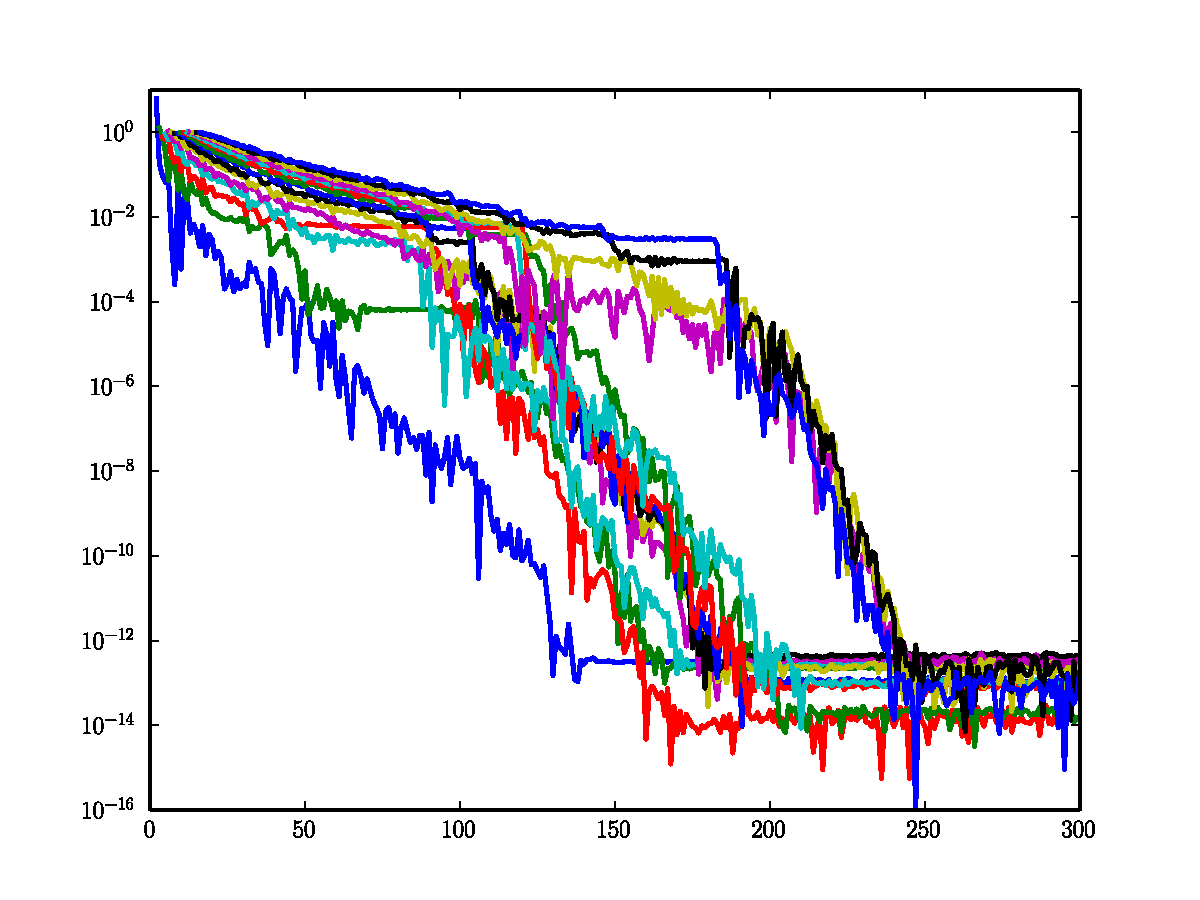
\includegraphics[width=\textwidth]{rand_eigs_conv.pdf}
\caption{The convergence of the Ritz Values to the largest eigenvalues of a matrix with random eigenvalues between $0$ and $1$.}
\label{fig:arnoldi_random_eig_conv}
\end{figure}

\begin{figure}
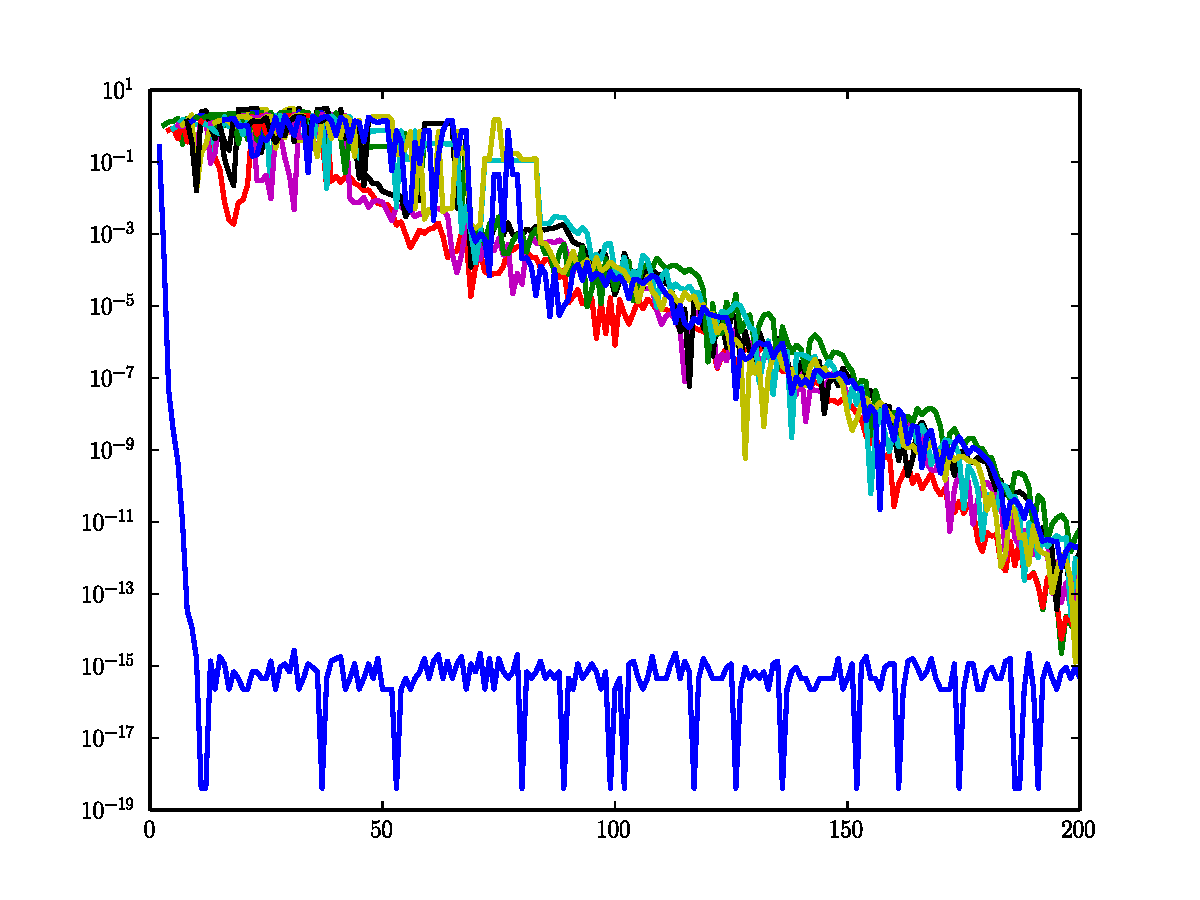
\includegraphics[width=\textwidth]{rand_vals_conv.pdf}
\caption{The convergence of the Ritz Values to the largest eigenvalues of a matrix with random values between $0$ and $1$.
Matrices of this form generally have a single isolated eigenvalue that is much larger than the rest.
It can be seen here that the Ritz Values converge to this eigenvalue much more quickly.}
\label{fig:arnoldi_random_val_conv}
\end{figure}

\begin{problem}
Run the Arnoldi Iteration on a random $100 \times 100$ array $A$.
Use a random vector as a starting point.
Find $H_{40}$ and compare the $10$ eigenvalues of largest magnitude of $H_{40}$ with the $10$ eigenvalues of largest magnitued of $A$.
Arnoldi Iteration is not the most effective way to work with dense matrices without significant patterns, but this example does illustrate the desired convergence.
\end{problem}

% Once the eigenvalue lab has been rewritten, have them use their own solver to find the eigenvalues of the $H_k$.

\section*{Lanczos Iteration}

Depending on the symmetry of the problem we may be able to make the Arnoldi Iteration more efficient.
Consider the case that $A$ is symmetric.
This means that the matrx $H$ is both Upper Hessenberg and symmetric, so it is tridiagonal.
Since $H$ is tridiagonal, in theory we should have that $A q_n$ is orthogonal to $q_0, \dots, q_{n-1}$.
This means that storage of all the columns of $Q_k$ is no longer necessary.
We can run the entire algorithm while storing only the previous column of $Q$ that we have computed.
We also can represent $H$ as two vectors: a vector $\alpha$ storing the values along the main diagonal of $H$, and a vector $\beta$ storing the values in the first subdiagonal (the values in the first superdiagonal are the same).
This change in the way things are stored allows Algorithm \ref{alg:arnoldi_iteration} to be simplified to Algorithm \ref{alg:lanczos_iteration}.
Algorithm \ref{alg:lanczos_iteration} is known as the Lanczos Iteration.

\begin{algorithm}
\begin{algorithmic}[1]
\Procedure{lanczos}{$b, Amul, k, tol=1E-8$}
	\State $q_0 \gets 0$								\Comment{Some initialization}
	\State $q_1 \gets \frac{b}{\|b\|_2}$
	\State $\alpha \gets \text{empty}\left(k\right)$
	\State $\beta \gets \text{empty}\left(k\right)$
	\State $\beta_{-1} = 0$
	\For{$j=0$, $j<k$}									\Comment{Perform the iteration.}
		\State $z \gets Amul\left(q_1\right)$					\Comment{$z$ is a temporary vector to store $q_{i+1}$.}
		\State $\alpha_i = q_1 \cdot z$						\Comment{$q_1$ is used to store the previous $q_i$}
		\State $z -= \alpha_i q_1 + \beta_{i-1} q_0$				\Comment{$q_0$ is used to store $q_{i-1}$}
		\If{$\beta_i<tol$}								\Comment{Stop if $\|q_{j+1}\|_2$ is too small.}
			\State \pseudoli{return} $\alpha [: i+1]$, $\beta [: i]$
		\EndIf
		\State $z /= \beta_i$
		\State $q_0, q_1 = q_1, z$						\Comment{Store new $q_{i+1}$ and $q_i$ on top of $q_1$ and $q_0$}
	\EndFor
	\State \pseudoli{return} $\alpha$, $\beta [: -1]$
\EndProcedure
\end{algorithmic}
\caption{The Lanczos Iteration}
\label{alg:lanczos_iteration}
\end{algorithm}

\begin{problem}
\label{prob:lanczos}
Write a Python function that performs the Lanczos Iteration.
Have it accept a starting vector $b$, a function $Amul$ that computes $A x$ for any vector $x$, a number $k$ of iterations to perform, and an optional argument $tol$ that defaults to \li{1E-8}.
\end{problem}

In its most basic form the Lanczos iteration is not very stable.
In exact arithmetic the vectors $q_i$ are exactly orthogonal, but in the presence of roundoff error this may be absolutely false.
In imprecise arithmetic it is possible for the $q_i$ to suffer from so much roundoff error that they mey no longer even be \textit{linearly independent}.
There are a variety of modifications to the Lanczos Iteration that address this instability.
The libraries used for Scipy use an algorithm called the Implicitly Restarted Lanczos Method.
We will not discuss these algorithms in detail here.
% If needed we could make a separate lab on the Lanczos Iteration and the Implicitly Restarted Lanczos Method.
% There isn't time or space here for it though.

\begin{problem}
The following code performs matrix multiplication by a tridiagonal symmetric matrix.
It accepts vectors $a$ and $b$ and $u$.
$a$ stores the entries in the main diagonal of the matrix.
$b$ stores the entries in the first sub/superdiagonal.
The function returns the image of $u$ under the matrix represented by $a$ and $b$.

\begin{lstlisting}
def tri_mul(a, b, u):
    v = a * u
    v[:-1] += b * u[1:]
    v[1:] += b * u[:-1]
    return v
\end{lstlisting}

Use the Lanczos Iteration function you wrote for Problem \ref{prob:lanczos} to estimate the $5$ largest eigenvalues of a symmetric tridiagonal matrix $A$ with random values in its nonzero diagonals (i.e. make $a$ and $b$) random.
For demonstration purposes, let $A$ be $1000 \times 1000$.
Perform $100$ iterations.
Compare the $5$ eigenvalues of largest absolute value with the $5$ Ritz Values of largest norm.
How do they compare?

Try running your simulation a few times for different vectors $a$ and $b$.
You may notice that, occasionally, the largest eigenvalue is repeated in the Ritz Values.
This happens because of the lack of orthogonality between the vectors used in the Lanczos Iteration.
These erroneous eigenvaleus are called "ghost eigenvalues."
They generally converge to actual eigenvalues of the matrix, but they can make the multiplicity of an eigenvalue look higher than it really is.
\end{problem}

% Have them code a version with a while loop that goes until convergence is reached. Use it to find the norm of random matrices.
% Point toward use of largest singular values in PCA and LSI in volume 3.

\section*{Polynomial root finding}

% Perform Arnoldi iteration on companion matrix. Give them a routine that computes Ax without explicitly constructing it.

% Plot basins of convergence for poynomial root finding.

\section*{Arnoldi Iteration in SciPy}

% Use it to find the Fiedler value to determine whether or not a graph is connected.


% Show Ghost Eigenvalues?

% Add another application if there's space.

% Eigvals of DFT computed via the FFT? This one is good because it uses the Lanczos iteration.

% Applications of eigenvalues of discretized representations of differential operators?